% -*-
\documentclass[12pt,letterpaper]{article}\usepackage[]{graphicx}\usepackage[]{color}
%% maxwidth is the original width if it is less than linewidth
%% otherwise use linewidth (to make sure the graphics do not exceed the margin)
\makeatletter
\def\maxwidth{ %
  \ifdim\Gin@nat@width>\linewidth
    \linewidth
  \else
    \Gin@nat@width
  \fi
}
\makeatother

\definecolor{fgcolor}{rgb}{0.345, 0.345, 0.345}
\newcommand{\hlnum}[1]{\textcolor[rgb]{0.686,0.059,0.569}{#1}}%
\newcommand{\hlstr}[1]{\textcolor[rgb]{0.192,0.494,0.8}{#1}}%
\newcommand{\hlcom}[1]{\textcolor[rgb]{0.678,0.584,0.686}{\textit{#1}}}%
\newcommand{\hlopt}[1]{\textcolor[rgb]{0,0,0}{#1}}%
\newcommand{\hlstd}[1]{\textcolor[rgb]{0.345,0.345,0.345}{#1}}%
\newcommand{\hlkwa}[1]{\textcolor[rgb]{0.161,0.373,0.58}{\textbf{#1}}}%
\newcommand{\hlkwb}[1]{\textcolor[rgb]{0.69,0.353,0.396}{#1}}%
\newcommand{\hlkwc}[1]{\textcolor[rgb]{0.333,0.667,0.333}{#1}}%
\newcommand{\hlkwd}[1]{\textcolor[rgb]{0.737,0.353,0.396}{\textbf{#1}}}%

\usepackage{framed}
\makeatletter
\newenvironment{kframe}{%
 \def\at@end@of@kframe{}%
 \ifinner\ifhmode%
  \def\at@end@of@kframe{\end{minipage}}%
  \begin{minipage}{\columnwidth}%
 \fi\fi%
 \def\FrameCommand##1{\hskip\@totalleftmargin \hskip-\fboxsep
 \colorbox{shadecolor}{##1}\hskip-\fboxsep
     % There is no \\@totalrightmargin, so:
     \hskip-\linewidth \hskip-\@totalleftmargin \hskip\columnwidth}%
 \MakeFramed {\advance\hsize-\width
   \@totalleftmargin\z@ \linewidth\hsize
   \@setminipage}}%
 {\par\unskip\endMakeFramed%
 \at@end@of@kframe}
\makeatother

\definecolor{shadecolor}{rgb}{.97, .97, .97}
\definecolor{messagecolor}{rgb}{0, 0, 0}
\definecolor{warningcolor}{rgb}{1, 0, 1}
\definecolor{errorcolor}{rgb}{1, 0, 0}
\newenvironment{knitrout}{}{} % an empty environment to be redefined in TeX

\usepackage{alltt}

%%%%% packages provided by sys bio template
\usepackage{fixltx2e}
\usepackage{textcomp}
\usepackage{fullpage}
\usepackage{amsfonts}
\usepackage{verbatim}
\usepackage[english]{babel}
\usepackage{pifont}
\usepackage{color}
\usepackage{setspace}
\usepackage{lscape}
\usepackage{indentfirst}
\usepackage[normalem]{ulem}
\usepackage{booktabs}
%\usepackage{nag}
\usepackage{natbib}
%\usepackage{bibtex}
\usepackage{float}
\usepackage{latexsym}
%\usepackage{hyperref}
\usepackage{url}
%\usepackage{html}
\usepackage{hyperref}
\usepackage{epsfig}
\usepackage{graphicx}
\usepackage{amssymb}
\usepackage{amsmath}
\usepackage{bm}
\usepackage{array}
%\usepackage{mhchem}
\usepackage{ifthen}
\usepackage{caption}
\usepackage{hyperref}
%\usepackage{xcolor}
\usepackage{amsthm}
\usepackage{amstext}
%%%%

% packages I need
\usepackage{authblk}
\usepackage{tabularx}
\usepackage{float}
\usepackage{amsmath}
\usepackage{longtable}
\usepackage[margin=1in]{geometry}
\usepackage[font=sf]{caption}

% Latex special characters are rendered correctly with XeTeX
\usepackage{xltxtra}
\usepackage{xunicode}
\defaultfontfeatures{Mapping=tex-text}

% Words are cut where needed
\usepackage{polyglossia}
\setdefaultlanguage[variant=american]{english}

% Use fancy fonts
\usepackage{fontspec}
\setmainfont[Mapping=tex-text]{Crimson Text}
\setsansfont{SourceSansPro-Regular}

% tables
\usepackage{multirow}

%%% syst bio options
\linespread{1.66}
% All text should be double-spaced
% with occasional exceptions for tables.
\raggedright
\setlength{\parindent}{0.5in}

\setcounter{secnumdepth}{0}
% Our sections are not numbered and our papers do not have
% Tables of Contents. We don't
% present a list of figures or list of tables, either.

% Any common font is fine.
% (A common sans-serif font should be used on figures, but figures should be
% separate from the LaTeX document.)

\pagestyle{empty}

\renewcommand{\section}[1]{%
\bigskip
\begin{center}
\begin{Large}
\normalfont\scshape #1
\medskip
\end{Large}
\end{center}}

\renewcommand{\subsection}[1]{%
\bigskip
\begin{center}
\begin{large}
\normalfont\itshape #1
\end{large}
\end{center}}

\renewcommand{\subsubsection}[1]{%
\vspace{2ex}
\noindent
\textit{#1.}---}

\renewcommand{\tableofcontents}{}

\bibpunct{(}{)}{;}{a}{}{,}  % this is a citation format command for natbib
%%% end syst bio options


\newcolumntype{b}{X}
\newcolumntype{s}{>{\hsize=.2\hsize}X}
\IfFileExists{upquote.sty}{\usepackage{upquote}}{}
\begin{document}

\begin{flushright}
Version dated: \today
\end{flushright}

\bigskip
\noindent CRYPTIC AND NOT-SO-CRYPTIC SEA CUCUMBER SPECIES COMPLEX

\bigskip
\medskip

\begin{center}
  \noindent{\Large \bf Cryptic and not-so-cryptic species in the complex
    ``\textit{Holothuria (Thymiosycia) imaptiens}'' (Forssk\r{a}l, 1775)
    (Echinodermata: Holothuroidea: Holothuriidae)}

\bigskip

\noindent{\normalsize \sc Fran\c{c}ois Michonneau}\\
\noindent {\small \it
$^1$Florida Museum of Natural History, University of Florida, Gainesville,
FL 32611-7800, USA}\\
\end{center}
\medskip

\noindent{\bf Corresponding author:} Fran\c{c}ois Michonneau, Division of
Invertebrate Zoology, Florida Museum of Natural History, Gainesville, FL
32611-7800, USA; E-mail: francois.michonneau@gmail.com\\


\vspace{1in}





\subsubsection{Abstract} Identifying accurately species is critical for our
understanding of patterns of diversity and speciation. However, for many
organisms with simple and variable morphological traits, the characters
traditionally used by taxonomists to identify species might lead to a
considerable under appreciation of their diversity. Recent advances in
molecular-data based computational methods have considerably improved our
ability to identify and test species limits. Here, we use an integrative
approach to delineate species in a complex of sea cucumbers. We used a
three-step approach to show that ``\textit{Holothuria impatiens}'', a common,
shallow-water species, occurring across the Indo-Pacific, the Western Atlantic
and the Mediterranean Sea, targeted locally by fisheries, is a complex of at
least 13 species. (1) We used the Generalized Mixed Yule Coalescent (GMYC) model
to identify putative species without \textit{a priori} hypotheses. In the
process, we also show that the number of putative species estimated with GMYC
can be affected considerably by the priors used to build the input tree. (2) We
assessed based on coloration patterns and distributional information, the most
relevant hypothesis. This approach allowed us to identify unambiguously 9
species. However, some of the lineages consistently assigned to belong to
different species using GMYC, are occurring in sympatry and are not
differentiated morphologically. (3) We used Bayes factors to compare competing
models of species assignment using the multispecies coalescent as implemented in
*BEAST. This approach allowed us to validate that the species identified using
GMYC were likely reproductively isolated. Estimates of the timing of
diversification also showed that these species diverged less than 2 Ma, which is
the fastest case of closely related species occurring in sympatry for a marine
metazoan. Our study demonstrates how clarifying species limits contribute to
refining our understanding of speciation.

\vspace{1.5in}


%% introduction

Despite challenges with definitions, species constitute the biological units
used to assess patterns of diversity, identify regions of conservation concern
and manage exploited resources \citep{Pimm2014}. For many taxonomic groups,
species limits are misunderstood and the level of undescribed diversity debated,
making global estimates of diversity poorly constrained
\citep{Appeltans2012,Costello2013}. Additionally, conservation efforts aim at
preserving the evolutionary potential of the species, but limited understanding
of the processes that maintain present and future diversity hinders these goals
\citep{Moritz2002}. Genetic data, and barcoding in particular, are facilitating
the documentation of biodiversity not only by providing an inexpensive and
efficient way to identify species and resolve complexes, but also by providing
insights into the evolutionary history of the species.

Barcoding has revealed that many species, thought to be well-understood, are
complexes. In most cases, these ``pseudo-cryptic'' species differ
morphologically but in traits not traditionally considered, or in traits not
available to taxonomists because of the preservation methods or the lack of
information about the natural history of the species \citep{Knowlton1993}. For
instance, differences in coloration \citep{Brown2007,Malay2010}, habitat
\citep{Prada2013}, or host preference \citep{Hebert2004}, were not considered as
indicative of species limits before cryptic lineages were uncovered by molecular
data. In these cases, the single-locus approach provided a way to infer species
limits using the evolutionary significant unit (ESU) concept \citep{Moritz1994}
that defines species-level units based on reciprocal monophyly in at least one
marker (typically mtDNA), and at least another defining attribute (morphology,
distribution, reciprocal monophyly in another trait). If this approach has
allowed to unravel high levels of unrecognized diversity, when other defining
attributes to infer reproductive isolation are lacking, the patterns of genetic
differentiation have remained difficult to interpret objectively.

Many species rely on chemical recognition systems to maintain species integrity
(e.g., mate recognition, habitat specificity) \citep{Knowlton1993}. Not only
these systems are poorly characterized or difficult to investigate in the
context of a taxonomic study, they also rarely translate into morphological,
behavioral or ecological differences. The absence of defining traits that
correlates with genetic clusters identified from single-locus data make these
species ``true cryptic'' complexes. New methods based on the multispecies
coalescent are emerging as powerful ways to investigate species limits in these
complexes when evidence is equivocal. By using multi-locus datasets, these
methods overcome some of the shortcomings of single-locus analyses that were
unable to distinguish between different processes leading to identical patterns
(e.g., incomplete lineage sorting and introgression), and do not depend on
arbitrary threshold of genetic divergence. Instead, they account for the
stochastic process associated with the independent sorting of genealogies along
the species tree, and use it to estimate the species tree and the demographic
history of the species \citep{Fujita2012a}. These methods also provide a
statistical framework to test competing species delineation hypotheses
\citep{Baele2012}.

Among marine organisms, the discovery of high levels of cryptic diversity has
challenged the importance of physical barriers as the primary driver of
diversification \citep{Mayr1954}. Since most marine invertebrates have a
potentially highly dispersive larval stage, and the oceans in general, and the
Indo-Pacific in particular, lack clear geographical barriers to dispersal,
opportunities for allopatric speciation seem limited. Yet, while many closely
related species have non-overlapping distributions suggesting that allopatric
speciation is prevalent, overlap in the distribution of sister species is
common. These observations have led to the realization that (1) selection (along
environmental gradients, sexual selection, host specificity) may play an
important role in reproductive isolation (reviewed in \citep{Bowen2013}); (2)
changes in species distributions have obscured the geographic context at the
time of speciation. By clarifying the identity of the species, by providing more
accurate estimates of the timing of speciation, and by estimating populations
sizes, the multispecies coalescent may shed light on the relative contribution
of these factors in shaping patterns of diversity, reveal new patterns and
refine our understanding of speciation in the sea.

In this study, we use coloration patterns, genetic, distributional and
ecological data, to unravel at least 13 species within ``\textit{Holothuria
  impatiens}'' (see column ``consensus'' in
Table~\ref{fig:species-limits}). This complex includes both species that can be
distinguished relatively easily from their live appearance, and species that can
only be identified genetically. The broad geographical distribution of this
complex and the elucidation of the phylogenetic relationships of its species
provide the opportunity to investigate the spatial and temporal dynamics of this
radiation.

Forssk\r{a}l described posthumously in 1775 \textit{Fistularia impatiens} from
material he collected in Suez, Egypt \citep{Forsskal1775}. The description is
limited, but indicates that the body wall is gray with dark spot, and with
well-developed, lightly colored tubercles. The drawing accompanying the
description corroborates these observations. Since then, the species has been
attributed to \textit{Holothuria}, the mostly reef-associated and most diverse
genus within the Holothuriidae. The range of \textit{H. impatiens} has been
extended, and today is recognized as the most widespread species in the
genus. Its range extends from the Red Sea through the entire Indo-West Pacific,
to the East Pacific, Caribbean and the Mediterranean. Pearson \citep{Pearson1915}
described \textit{Thymiosycia} as one of five subgenera in \textit{Holothuria},
and designated \textit{Holothuria impatiens} as the type species. The modern
concept of \textit{Thymiosycia} was proposed by Rowe \citep{Rowe1969} to include
13 species.
% characterized by well developed, regular and symmetrical tables and buttons.

\textit{Holothuria impatiens} is a common, to locally abundant species found
under rocks (in particular in lagoons and back-reef habitats), and is largely
restricted to shallow water (< 10~m), although it has been recorded down to
158~m (Y. Samyn, pers. comm.).  Because of its ubiquitous distribution, it is
one of the more studied species in the family with studies on its reproduction
\citep{Harriott1985}; Cuvierian tubules \citep{Flammang2002,Becker+Flammang2010};
toxicity \citep{Bakus1974}; feeding preferences \citep{Roberts1982}; parasites
\citep{Martens1994}; the chemical composition, statistical analysis of the shape,
and ontogenic changes in ossicles \citep{Hampton1958,Hampton1959,Cutress1996}. It
has also been included in molecular phylogenies that investigated relationships
among the major groups of holothurians (e.g., \citep{Lacey2005}) or as an
outgroup when studying relationships within a sub-genus (e.g.,
\citep{Honey-Escandon2012}). \textit{Holothuria impatiens} is a low-value
commercial species that is fished in the Eastern Pacific
\citep{Toral-Granda2008}, Madagascar \citep{Conand2007}, and Palau
\citep{Pakoa2009}.

Despite its relative biological and commercial importance, the variation
observed in color patterns reported by previous workers (e.g.,
\cite[p.178]{Clark1921}, \citep{Rowe+Richmond2004}) has yet to be
investigated. The goal of this study is to identify cryptic species in the
``\textit{Holothuria impatiens}'' complex, and to understand the temporal and
spatial dynamics of its diversification. To this end, we sampled the entire
known geographic range of this complex, and assembled a multi-locus dataset.

To identify species limits in the complex, we used a combination of
complementary methods of species delineation following modifications of the
approaches outlined by \citep{Leache2010,Satler2013,Grummer2014}. First, we used
the Generalized Mixed Yule Coalescent method (GMYC) on a portion of the
mitochondrial locus COI to delineate putative species
\citep{Pons2006,Monaghan2009}. We then used independent lines of evidence (color
patterns, ecology and geographic information) to assess the validity of these
putative species. When no other line of evidence could separate the putative
species identified with GMYC, we used model comparison in *BEAST
\citep{Heled2010,Baele2012} to validate species limits. Our study shows that
these methods can be added to the lines of evidence typically used in
integrative taxonomy, and provide a powerful tool for evaluating species limits
in rapidly evolving groups with limited morphological and genetic
differentiation.

%% need something here about how many species we find, how they are related to
%% each others, and how in this paper we test how methods perform to our
%% "perception?" of what the species are.

\section{Methods}

\subsection{Sampling}

Specimens were collected at low tide, on snorkel, on SCUBA or by dredging. Most
specimens were photographed while alive \textit{in situ} or in the lab,
anesthetized in a 1:1 solution of sea water and 7.5\% solution of magnesium
chloride hexahydrate, then preserved in 75\% ethanol. When possible, tentacles
were clipped, immediately put in 95-99\% ethanol, and later used for DNA
extractions.

Specimens were deposited in the Invertebrate Zoology collections of the Florida
Museum of Natural History, University of Florida (UF), Gainesville, FL, USA,
while tissue samples are stored in the Genetic Resources Repository of this
museum. A few additional tissue samples were taken from vouchers housed at other
institutions or were obtained through collaborators without vouchers being
retained (Table~\ref{tab:specimen-table} for details).

We examined 219 specimens morphologically and
208 were used for molecular analyses. These specimens were
collected across the entire known range of \textit{H. impatiens}: Mediterranean
Sea, Caribbean Sea, Red Sea, tropical Indian and Pacific Oceans
(Table~\ref{tab:specimen-table}).


\subsection{DNA extraction and amplification}



DNA was extracted using either Invitrogen$^{\text{TM}}$ DNAZol\textregistered\
or Omega Bio-Tek$^{\text{TM}}$ E.Z.N.A\textregistered\ Mollusc DNA kit following
manufacturer recommendations. DNA was most often extracted from tentacles,
sometimes from gonads, longitudinal muscles or body wall. When possible, the
extractions were performed on tissue sampled in the field.

In this study we amplified the mitochondrial markers COI, 16S, ATP6 and the
nuclear markers histone 3 (H3a), 18S, ITS1-5.8S-ITS2, c0036 and c0775
(Table~\ref{tab:pcrConditions}). ATP6 primers were developed in this study based
on sequences available for this locus in GenBank. c0036 and c0775 are anonymous
markers developed from a 454 run on genomic DNA from \textit{Holothuria edulis}.
These loci were identified using blastx on the contigs obtained from the 454 run
against the predicted proteins for the sea urchin \textit{Strongylocentrotus
  purpuratus} genome. c0036 matches a portion of the gene encoding for an
histone H3-like centromeric protein A-like (locus XP\_003723879), with an
e-value of 2.10$^{-43}$. c0775 matches a portion of the gene encoding for the
protein SFI1 (locus XP\_792620), with an e-value of 3.10$^{-16}$.

Primers and PCR conditions used are provided in
Table~\ref{tab:pcrConditions}. Because of the length of ITS1-5.8S-ITS2, we used
the additional sequencing primer fm-5.8S-f. The primer fm-ITS-f is the reverse
complement sequence of the primer 18S-1708R (WN-1708R in \citep{Lacey2005}), and
fm-ITS-r is the reverse complement of LSUFW1 (LSU D1,D2 fw1: 56-74 in
\citep{Sonnenberg2007}).

We conducted PCR in 25$\mu$L reactions using either 15.4~$\mu$L of water,
2.5~$\mu$L of Sigma-Alrich \textregistered 10X PCR buffer, 2.5~$\mu$L of dNTP,
2~$\mu$L of MgCl$_2$, 1~$\mu$L for each of the forward and reverse primers (at
10 mM), and 0.1~$\mu$L of Sigma-Aldrich\textregistered Jumpstart$^{\text{TM}}$
Taq DNA polymerase or the Promega GoTaq MasterMix following manufacturer
recommendations.

Sequencing of PCR products was performed by the Interdisciplinary Center for
Biotechnology Research at the University of Florida. Chromatrograms were edited
using Geneious \citep{Geneious558}.

Overall, 84 positions
(1.14\% of the alignment length,
and 0.02\% of the total number of
nucleotides in the alignment) contained heterozygous positions. We used the
International Union of Pure and Applied Chemistry (IUPAC) nomenclature codes for
these positions in the alignment, which are considered as missing data by all
the software used in this study.

\begin{table}
  \caption{Primers and PCR conditions for the markers used in this study. Temp:
    annealing temperature, Cycles: number of PCR cycles used to amplify the
    locus, Ref.: reference used for the primers.}
\begin{tabular}{ l l p{6cm} l l p{2cm}}
  \hline
  Marker & Primer & Primer Forward ($5'-3'$) \& Primer Reverse ($5'-3'$)  & Temp &  Cycles & Ref. \\
  \hline
  % COI ---
  COI &  COIceF  & ACT GCC CAC GCC CTA GTA ATG ATA TTT TTT ATG GTN ATG CC & 42 & 40 & \citep{Hoareau2010} \\
       & COIceR  & TCG TGT GTC TAC GTC CAT TCC TAC TGT RAA CAT RTG & & & \\
  % 16S ---
  16S & 16SAR & CGC CTG TTT ATC AAA AAC AT & 52 & 35 & \citep{Arndt1996} \\
      & 16SBR & GCC GGT CTG AAC TCA GAT CAC GT & & & \\
  % 16Sc ---
  %% TODO
  % ATP6 ---
  ATP6 & ATP6f   & GGA CAA TTT TCC CCA GAC CT & 42 & 40 & This study \\
       & ATP6r   & GGT GAA GAG GGT GTT GAT GG & & & \\
  % 28S ---
  28S  & LSUFW1  & AGC GGA GGA AAA GAA ACT A &  42 & 40 & \citep{Sonnenberg2007} \\
       & LSUREV2 & ACG ATC GAT TTG CAC GTC AG & & & \\
  % ITS ---
  ITS1-5.8S-ITS2  & fm-ITS-f  & AGG TGA ACC TGC AGA TGG ATC A & 45 & 40 & This study, \citep{Lacey2005,Sonnenberg2007} \\
                  & fm-5.8S-f & CGT CGA TGA AGA ACG CAG YW & & & \\
                  & fm-ITS-r  & TAG TTT CTT TTC CTC CGC T  & & & \\
  % c0036 ---
  c0036 & c0036f & TAA CGA CGG ATC TCA CGG AG & 42 & 45 & This study \\
        & c0036r & AAT AAT GCT GGC GTG ACG TC & & & \\
  % c0775 ---
  c0775 & c0775f & GCT CTT CGT TCA ATT TAT CTC GC & 42 & 40 & This study \\
        & c0775r & GGG ATG CAG TTT GTC GAG TG & & & \\
  \hline
\end{tabular}
\label{tab:pcrConditions}
\end{table}

\subsection{Definitions}

In this paper we use three concepts: ``putative species'', ``evolutionary
significant units (ESUs)'', and ``species'':

\begin{itemize}
\item ``Putative species'' describes the lineages identified by the GMYC method
  and follows the terminology used by the authors of the method \citep{Pons2006,
    Monaghan2009}.
\item ``Evolutionary significant units (ESUs)'' are defined as reciprocally
  monophyletic lineages in COI that are also characterized by another
  independent defining attribute (e.g., coloration, morphology, geographical
  distribution, reciprocal monophyly in another marker). We use this concept
  as defined by Moritz \citep{Moritz1994}.
\item The ``species'' are the lineages supported by the model of species
  delineation that best explains the data as assessed by Bayes factors estimated
  from the multispecies coalescent in *BEAST. They provide an indirect
  assessment of reproductive isolation and the species are assumed to not
  exchange genes, forming independent distinct lineages.
\end{itemize}

\subsection{Species limits with GMYC}

To delineate putative species based on molecular data, we fit the generalized
mixed Yule coalescent (GMYC) model (\citep{Pons2006,Monaghan2009,Fujisawa2013})
to the COI sequence data. This approach attempts to detect transitions in the
branching rate of an ultrametric tree corresponding to the expected increase in
lineage accumulation resulting from the shift between speciation and
population-level coalescent events. To determine the location of the threshold,
the GMYC model is fit at different nodes along the tree, and the one that
provides the best likelihood for the location of the switch is
selected. Lineages found beyond this threshold are considered different species.

To obtain the ultrametric trees required by this method, we used BEAST as it
provides a powerful statistical framework to interpret the chronological context
of molecular variation \citep{Drummond2014}. Despite some investigations of the
effects of priors on the number of species estimated by GMYC
(\citep{Monaghan2009, Fujisawa2013, Talavera2013}), we here revisit the impact of
specifying a strict or a log-normal relaxed clock, as well as the type of tree
prior used (coalescent with constant population size \citep{Kingman1982},
coalescent with exponentially growing population size \citep{Griffiths1994}, and
Yule \citep{Yule1925}). The type of clock used will affect branch lengths, it is
however difficult to predict \textit{a priori} how the misspecification of this
parameter will influence the results. Monaghan et al \citep{Monaghan2009}
indicate that using a coalescent constant tree prior is a more conservative
approach compared to using a Yule prior, as GMYC uses the coalescent as the null
model to explain the branching pattern. Their results validated their
predictions and the GMYC method detected more species on trees estimated with a
Yule prior. However, these results might be influenced by the nature of the
data, in particular by the amount of variation observed in the sequences, and
deserve further testing.

To our knowledge few studies have investigated the effect of retaining identical
haplotypes in the analysis (but see \citep{Talavera2013}). In other studies,
identical sequences were removed as they were thought to make the task of
estimating the transition problematic \citep{Monaghan2009}, as the GMYC method
cannot accommodate for the null branch lengths associated with identical
sequences \citep{Fujisawa2013}. Contrary to other programs, BEAST does not assign
zero edge length to terminal branches for identical sequences, and thus allows
retaining them in the analysis. There are obvious theoretical advantages for
retaining identical sequences: BEAST assumes that the sequences represent a
random sample of the population when estimating effective population
sizes. Removing identical sequences will lead to spuriously high levels of
genetic diversity, in turn leading to overestimating population sizes
\cite[p.98]{Drummond2014}. As population sizes directly influence the
probability that lineages will coalesce, removing identical sequences will lead
to longer branches in the trees, blurring the distinction between interspecific
and intraspecific coalescent events. We can therefore predict that removing
identical sequences of the analysis will lead to higher number of species
detected by GMYC and higher uncertainty, both of which are undesirable for the
purpose of the analysis.

We performed the GMYC analyses using only COI sequences as the method was
designed to be used on single locus datasets, and we wanted to compare how our
conclusions might differ if the entire dataset was considered. COI genealogies
were estimated using BEAST 1.8.0 \citep{Drummond2012} and BEAGLE 2.1
\citep{Ayres2012}. To determine the optimal partition scheme, we used
PartitionFinder \citep{Lanfear2012} on the dataset including all sequences as
well as on the dataset limited to distinct haplotypes only. We performed a
complete search using each codon position as a partition, and limiting the
search to the JC, HKY and GTR models with or without a proportion of invariant
sites (+I) and/or gamma-distributed rates of evolution (+G) (12 different models
\textit{in toto}). Both datasets (all sequences, only haplotypes) favored to
assign each codon position to independent partitions. The partition scheme
selected by PartitionFinder led to poor mixing due to over-parametrization in
initial test runs. We modified the partition scheme slightly, to use: HKY+I+G,
GTR+G and HKY for each codon position respectively for the dataset including all
sequences; and HKY+G, HKY+G and HKY for the analyses on unique haplotypes. In
all analyses, base frequencies were estimated.

We used a log-normal distribution as the prior for the mean rate of substitution
for the log-normal relaxed clock and the strict clock, with a \textit{log}(mean)
of -4 and a \textit{log}(standard deviation) of 1.

As no fossils are known in \textit{Holothuria}, we used the closure of the
isthmus of Panama to calibrate the clock. The isthmus of Panama was completely
closed about 3 Ma but most species were probably isolated earlier
\citep{Lessios2008}. We chose a conservative estimate to account for the fact
that the sister species lineages found across the isthmus are the lineages found
in the Galapagos and the Caribbean (the coastal Eastern Pacific lineage is
sister to the one found in the Galapagos, Fig.~\ref{fig:impatiens-tree}). We
constrained the age of the node corresponding to the most recent common ancestor
of the individuals found in the Galapagos archipelago, the coast of the Eastern
Pacific and in the Caribbean using a log-normal prior with a \textit{log}(mean)
of 1.5, a \textit{log}(standard deviation) of 0.75 and an offset of 2.5. This
distribution translates into a mean age of divergence of
6.98 millions years ago
(Ma), (95\% confidence interval of [3.53, 21.99]).

We set the MCMC chain lengths at 5.10$^{7}$, sampling every 5.10$^{3}$
generations. All analyses were run twice from independent starting points and
were checked for convergence. From visual inspection of the values sampled by
the chains with Tracer 1.6, we determined that a burnin of 10\% was sufficient
for all runs. ESS values for all parameters were above 350 in each independent
run, and the samples from the posterior from each runs were combined.

The trees sampled from the posterior were summarized with treeannotator using
the common ancestor tree method, as this method provides a more accurate
estimate of the divergence times from the trees sampled from the posterior
compared to the other methods available in treeannotator \citep{Heled2013}.

These trees were used to fit the single-threshold (\citep{Pons2006}) and the
multi-threshold \citep{Monaghan2009} GYMC model using the R package splits 1.0-19
\citep{Ezard2013}. We considered the number of ``entities'' returned by GMYC as
the estimated number of species in our analyses. The confidence interval for the
number of species corresponds to the minimum and maximum numbers of species for
threshold values found within 2 log-likelihood units of the threshold associated
with the highest likelihood.

\subsection{Species limits with coloration and geography}

To determine whether the putative species delineated with GMYC were biologically
sound, we investigated their color patterns, geographical distribution and ecology.

Coloration information was obtained from the photographs of the live specimens
and from field observations. Ecological and geographical coordinates were
retrieved from the collecting information associated with the specimens.

%% To compare intra- and inter-specific variation in ossicle size and shape in the
%% dorsal body wall, we measured various characteristics of buttons and tables
%% composing the ossicle assemblage of \textit{Holothuria impatiens}
%% (Fig.\ref{fig:ossicleMeasurements}).

%% For 3-5 individuals of each ESU, we measured characteristics of at least 10
%% buttons and 10 tables. Measurements were made from  photographs of the
%% ossicles at 400x magnification using ImageJ (\ref{ImageJ}).

%% Measurements were analyzed in a principal component analysis in R
%% \ref{Rcoreteam}.

\subsection{Species limits with *BEAST}

Some of the putative species delineated by GMYC form well defined but shallow
clusters, have geographically defined ranges, but cannot be differentiated
morphologically. Their ranges overlap (e.g., \texttt{Hawaii}, \texttt{Wpac}) or
border (e.g., \texttt{RedSea}) the widespread \texttt{ESU1}, bringing into
question the reproductive isolation of these lineages. To test whether these
clusters are reproductively isolated, we compared competing hypotheses of
species delineation with *BEAST v 1.8.0 \citep{Heled2010} using Bayes factors
(BF) estimated by the stepping-stone (SS) and the path sampling (PS) methods
\citep{Baele2012}.

*BEAST infers the species trees from a multi-locus dataset using the
multispecies coalescent in a Bayesian framework to account for intraspecies
polymorphism and incomplete lineage sorting. This method assumes reproductive
isolation (absence of gene flow) among species and requires the assignment of
individuals to species \textit{a priori}.

Bayes factors (BF) provide a powerful framework for model selection by comparing
marginal likelihoods. The models do not have to be nested and the complexity of
the models is directly accounted for by the marginal likelihoods
\citep{Baele2012}. Kass \& Raftery \citep{Kass1995} developed guidelines to
interpret BF values such that $2.ln(B_{01})$ (where $B_{01} =
\frac{p(Y|M_1)}{p(Y|M_0)}$ with $Y$ is the observed data and $M_i$ the model
under consideration) must be $> 6$ to consider the evidence ``strong'' for (or
against) the null hypothesis, and $> 10$ to consider it ``very strong''. Here,
we used PS and SS methods to estimate and compare the marginal likelihoods
$p(Y|M)$ of alternative assignments of individuals to species in *BEAST. With
this approach, we tested whether we could detect the signature of reproductive
isolation among individuals assigned to different putative species by GMYC but
that cannot be teased apart based on color patterns or other evidence.

We investigated whether *BEAST favored models where all or some of the following
ESUs were considered distinct species: \texttt{WPac}, \texttt{Hawaii} and
\texttt{RedSea}, or were panmictic with \texttt{ESU1} (Table
\ref{tab:delineationModels}). We included \texttt{ESU3} and \texttt{gracilis} in
our analysis to allow the estimation of the topology when all individuals for
the species tested where attributed to \texttt{ESU1}. The null hypothesis was
that all putative species were reproductively isolated.



In these analyses, we selected individuals for which we had at least one
mitochondrial marker and one nuclear marker (43
individuals: 9 of \texttt{ESU1},
7 of \texttt{Hawaii}, 7 of
\texttt{Wpac}, 5 of \texttt{RedSea},
7 of \texttt{gracilis}, 8 of
\texttt{ESU3}). We used data from the following markers: 16S, COI, ATP6, c0036,
c0775, ITS, LSU and H3a; and the same approach as for the phylogeny of the
entire complex (see below): using Gblocks to remove ambiguous parts of the
alignment in ITS, PartitionFinder to find the most appropriate partition scheme
and models of molecular evolution. We unlinked clocks for all markers, used
strict molecular clocks, fixing the COI clock at 1\%.million years$^{-1}$ which
is the rate estimated from the analyses on COI used for the GMYC analyses. The
rate for the other clocks were estimated relatively to the COI clock. We ran at
least two independent runs for 50.10$^{6}$ generations for each group.

\begin{table}
  \centering
  \caption{Species groupings used in models of species delineation.}
  \begin{tabular}{ l l l }
    \hline
    Model   & Number of species & ESUs attributed to ESU1 \\
    \hline
    M0      &     5             &  --                     \\
    M1      &     2             &  \texttt{Wpac}, \texttt{Hawaii}, \texttt{RedSea}   \\
    M2      &     3             &  \texttt{Wpac}, \texttt{RedSea}           \\
    M3      &     3             &  \texttt{Wpac}, \texttt{Hawaii}           \\
    M4      &     4             &  \texttt{Wpac}                   \\
    M5      &     4             &  \texttt{Hawaii}                 \\
    M6      &     4             &  \texttt{RedSea}                 \\
    \hline
  \end{tabular}
  \label{tab:delineationModels}
\end{table}

For the estimation of the marginal likelihoods, we used the settings recommended
by Baele et al \citep{Baele2012} with path steps of 100, and sampling along
evenly spaced quantiles of a $Beta(0.3, 1)$ distribution, but increased the
chain lengths to 3.10$^{6}$. We interpreted an absolute difference between the
marginal likelihoods estimated with the stepping stone and the path sampling
methods higher than 1 as a failure of the estimates to converge. In these cases,
we repeated the analysis from a different starting point until the difference
between the likelihoods was less than 1.

To rule out that this approach did not favor models that included more species,
we added a ``ghost'' species in the analysis. This ``ghost'' species was
comprised of individuals that formed a shallow reciprocally monophyletic group
in COI within \texttt{ESU1}, but that was not identified as a putative species
in any of the sGMYC analyses.

To confirm that COI, which was used to delineate putative species with GMYC, did
not drive the differences in marginal likelihoods among the models tested with
*BEAST, we repeated some of the analyses omitting COI (models M0 and M4-M6 in
Table~\ref{tab:delineationModels}). We also repeated the analyses for these
models using only nuclear data to assess the influence of mitochondrial data on
the results.

% TODO -- Furthermore, to assess more generally the contribution of the nuclear
% data to the results, we repeated the analyses by attributing randomly the
% nuclear data.


\subsection{Phylogeny and divergence time estimation}

Sequences obtained for each marker were aligned using MUSCLE \citep{Edgar2004}
with the default settings. All markers led to unambiguous alignments except for
ITS. For this locus, we used Gblocks \citep{Castresana2000} to remove parts that
were difficult to align using a minimum length of a block of 5 (\texttt{-b4=5}),
and the option ``all gap positions can be selected'' (\texttt{-b5=a}). We used
the resulting alignment to estimate the phylogenetic relationships and the
timing of the divergence among the different lineages of \textit{Holothuria
  impatiens} using RAxML 8.0.1 \citep{Stamatakis2014} and BEAST 2.1.2
\citep{Bouckaert2014} (with BEAGLE 2.1.2 \citep{Ayres2012}).

To determine the optimal partition scheme and models of molecular evolution, we
analyzed the alignment using PartitionFinder \citep{Lanfear2012}. We defined the
data blocks such that the three codon position for ATP6, COI, H3a, and each of
16S, c0036, c0775, ITS and LSU were individual partitions. We used the greedy
algorithm, with linked branch lengths, no user tree, and models of molecular
evolution available by default in BEAST (JC69, HKY, GTR, without or with a
proportion of invariant sites [+I] and/or Gamma distributed rates across sites
[+G]). We selected the best-fit models and partition schemes based on the
Bayesian Information Criterion. The best fit model had 9 partitions.

For the BEAST analysis, following some initial testing runs, we modified the
partition scheme slightly to improve mixing of the chains as the partition
scheme selected by PartitionFinder led to over-parametrization (Table
\ref{tab:sm-partitions}).

We used three independent strict molecular clocks (one for each of mitochondrial
markers, protein-coding nuclear markers, nuclear ribosomal markers)
\citep{Hasegawa1985}. The tree prior was set to a Yule process, and a random
starting tree. The Markov chains were run for 185.10$^6$ generations (and
sampled every 5.10$^3$ generations). The analysis was repeated twice from
independent starting points.

We used Tracer 1.6 to check that the MCMC chains had reached stationarity, that
mixing was adequate, and that the two independent runs were consistent. We
ensured that a representative sample of the posterior distributions was sampled
for each independent runs, by checking that the ESS values for all parameters
were above 200. The samples from the posterior distribution from both runs were
combined using logcombiner after removing a 20\% burnin, resulting in 29601
states sampled. The ESS values obtained by combining the runs were all above
440. We summarized the trees sampled with treeannotator using the common ancestor
tree method \citep{Heled2013}.



\section{Results}

\begin{figure}
  \centering
    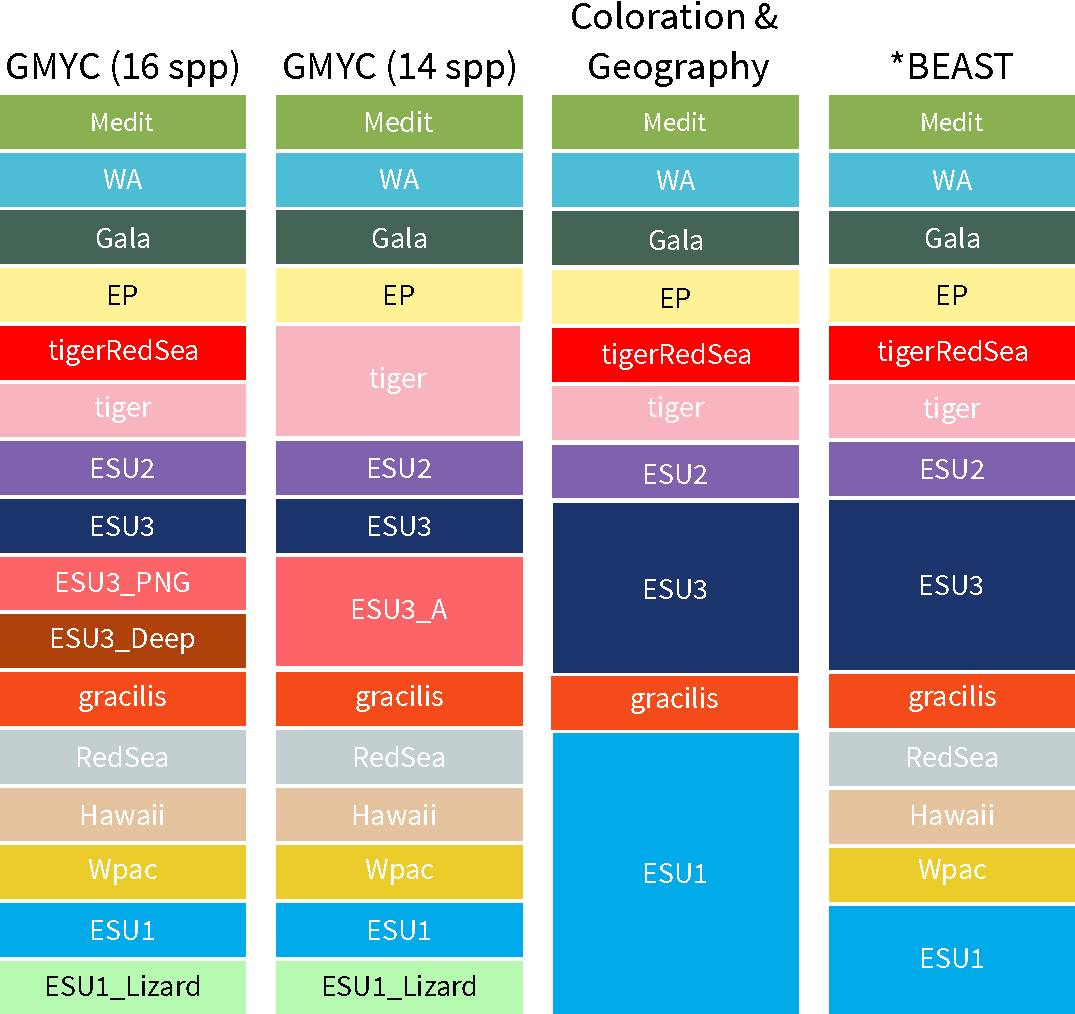
\includegraphics[width=6.5in]{figures-manual/species_limits.pdf}
    \caption{Correspondence between the different criteria used to delineate the
      species of the ``\textit{Holothuria impatiens}'' complex. Medit:
      Mediterranean, WA: Western Atlantic, Gala: Galapagos, EP: Eastern Pacific;
      PNG: Papua New Guinea; Wpac: Western Pacific.}
    \label{fig:species-limits}
\end{figure}

\subsection{Sequence data}




The complete sequence data set was 5966~bp (with
2505~bp from mitochondrial
genome, and 3461~bp from the nuclear genome,
Table~\ref{tab:loci-characteristics}). Of the 1220
parsimony-informative sites, 69\% were from the mitochondrial loci
(Table~\ref{tab:loci-characteristics}).


% latex table generated in R 3.2.0 by xtable 1.8-0 package
% Fri May 22 16:50:19 2015
\begin{table}[ht]
\centering
\caption{Characteristics of the loci used for the phylogenetic analyses. $N$: number of individuals sequenced, $K$: number of unique sequences, bp: length of the aligned (unaligned) sequences, $S$: number of segregating sites, $S_{i}$: number of parsimony informative sites. The statistics given for ITS are for the ones used in the analysis (i.e., after using Gblock).} 
\label{tab:loci-characteristics}
\begin{tabular}{rllllllll}
 & \multicolumn{3}{c}{mtDNA} & \multicolumn{5}{|c}{nucDNA} \\ 
\cline{2-4} \cline{5-9}
 & 16S & COI & ATP6 & c0036 & c0775 & H3a & ITS & LSU \\ 
  \hline
$N$ & 94 & 203 & 64 & 70 & 59 & 39 & 61 & 6 \\ 
  $K$ & 94 & 203 & 59 & 70 & 23 & 34 & 61 & 6 \\ 
  bp & 1179 (1117) & 673 (655) & 653 (653) & 637 (624) & 282 (282) & 334 (334) & 1085 (1040) & 1123 (1072) \\ 
  $S$ & 479 & 219 & 330 & 140 & 47 & 46 & 419 & 201 \\ 
  $S_{i}$ & 383 & 198 & 265 & 97 & 28 & 5 & 237 & 7 \\ 
   \hline
\end{tabular}
\end{table}



We obtained sequence data from 207 individuals covering the entire known geographical
range of \textit{Holothuria impatiens}. All of these individuals were
sequenced for at least one mitochondrial locus, and
36\% were
sequenced for at least 1 nuclear locus and
34\% for 2 or more
(Fig.~\ref{fig:loci-coverage-plot}).

% Here comment on results based on RAxML runs on individual loci.


\subsection{Species limits with GMYC}





The maximum-likelihood estimates for the number of putative species varied
widely and ranged from 14 to 20 for the
single-threshold method (sGMYC), and from 17 to 23
for the multi-threshold method (mGMYC) (Fig~\ref{fig:gmyc-coi-plot}).


\begin{figure}
  {\centering \includegraphics[width=\maxwidth]{figures-remake/gmyc-coi-plot.pdf}}

  \caption{Number of species estimated by single and multi-threshold GMYC
    methods on COI phylogenies. The dots represent the number of species
    associated with the node(s) that correspond(s) to the highest likelihood(s)
    for the location of the shift(s), the dotted lines represent the range for
    the estimated number of species for nodes within 2 likelihood units of the
    maximum-likelihood estimate.}\label{fig:gmyc-coi-plot}
\end{figure}


Species estimates from sGMYC were more conservative and with narrower confidence
intervals (CI) than the mGMYC approach. The maximum-likelihood estimates for the
sGMYC were in most cases at the lower limit of the CI, while the estimates from
the mGMYC were at the upper limit. For the analyses performed on all the
sequences, the CI for the estimated number of species using sGMYC and mGMYC did
not overlap.

On the genealogies estimated with a strict clock, sGMYC was less sensitive to
the type of tree prior used, as the estimated number of species was identical
for the three priors tested with 16 and
17 estimated species for analyses on all
haplotypes and on unique haplotypes respectively. The Yule prior produced equal
or more conservative estimates of the number of species compared to the two
types of coalescent priors.

With sGMYC, the estimated number of species was more conservative and less
sensitive to the priors used to reconstruct the genealogy when all sequences
were included.

Overall, the putative species delineated with sGMYC were consistent across the
different priors used. For the analyses based on all sequences, the difference
between the 14 species estimated with the Yule prior and the 16 species
estimated with the other priors was caused by (1) the lumping of
\texttt{tigerRedSea} and \texttt{tiger}; (2) the later time to coalescence for
divergent haplotypes related to \texttt{ESU3} with the Yule prior.

For the analyses based on unique haplotypes and a relaxed clock, with the Yule
prior, the coalescence of the haplotypes happened later in the tree leading to
lower estimated number of species compared to the coalescent priors. With the
relaxed clock, many coalescent events were reconstructed in the vicinity of the
threshold leading to broad confidence intervals.

With the strict clock analyses, the additional species delineated between the
unique haplotypes and all sequences corresponds to the recognition of both
\texttt{tiger} and \texttt{tigerRedSea}.

For all analyses, at least one putative species was represented by a single
sequence. A divergent lineage related to \texttt{ESU1}, collected in Lizard
Island, Australia, was assigned to its own species (\texttt{ESU1\_Lizard} in
Fig.~\ref{fig:species-limits}). In all analyses (except with the most
conservative estimate, i.e., using all sequences, a relaxed clock and a Yule
prior), two sequences related to \texttt{ESU3} (from the Ryukyus, Japan, and
from Papua New Guinea), were each assigned to their own species
(\texttt{ESU3\_Deep} and \texttt{ESU3\_PNG} respectively in
Fig.~\ref{fig:species-limits}).

\subsection{Species limits with coloration and geography}

Members of the ``\textit{H. impatiens}'' complex are characterized by two
dominant colors. The dark coloration is typically solid towards the anterior
end, forms bands in the middle of the body, and then spots that become rare
towards the posterior end.  This pattern varies considerably across species and
across individuals. The dark color is typically brown but varies in lightness
and can take a red or purple tint. The lighter color is typically gray but
varies in lightness from light brown to yellow or even white. The light-colored
areas typically harbor a ``salt-and-pepper'' pattern with small dark spots on
the light background. Despite these common characteristics, the combination of
color patterns and geographical distribution allows us to distinguish
unambiguously at least ten species (Fig.~\ref{fig:species-limits},
\ref{fig:photo-ESU1-andFriends}, \ref{fig:photo-ESU2-andFriends}).

\texttt{Medit}, \texttt{WA}, \texttt{Gala}, \texttt{EP}, \texttt{ESU1} have
similar color patterns but subtle differences, and the restriction of their
ranges to an oceanic basin or an archipelago allow teasing them
apart. \texttt{ESU2} is the only species with bright yellow papillae and
tentacles (Figure~\ref{fig:photo-ESU2-andFriends}). \texttt{tiger} and
\texttt{tigerRedSea} are also very distinctive with sparse, dark, tubercles that
barely raise from the body wall, giving them a smoother appearance than the
other species. They are also much larger than the other species and specimens
reach regularly more than 30~cm. \texttt{gracilis} has very large, conical,
typically red tubercles, and a very distinctive ``gritty'' texture.
\texttt{ESU3} has elongated, pyramidal tubercles with white papillae. However,
\texttt{ESU1}, \texttt{Hawaii} and \texttt{Wpac} have broadly overlapping
distributions and are morphologically indistinguishable
(Figure~\ref{fig:photo-ESU1-andFriends}).

\begin{figure}
  \centering
    \includegraphics[width=6.5in]{figures-manual/figure-group1.jpg}
    \caption{Dorsal view of members of the ``\textit{Holothuria impatiens}''
      complex. A. ESU1, R\'{e}union Island, UF6487; B. ESU1, R\'{e}union Island,
      UF6588; C. ESU1, Majuro, Marshall Islands, UF6748; D. ESU1, Okinawa, Japan, UF10950;
      E. RedSea, Djibouti, UF12070; F. Wpac, Majuro Marshall Islands, UF6771;
      G. Hawaii, French Fregate Shoal, Hawaiian archipelago, UF6243.}
    \label{fig:photo-ESU1-andFriends}
\end{figure}

\begin{figure}
  \centering
    \includegraphics[width=6.5in]{figures-manual/figure-group2.jpg}
    \caption{Dorsal view of members of the ``\textit{Holothuria impatiens}''
      complex. A. ESU2, Nosy B\'{e}, Madagascar, UF7287 (juvenile); B. ESU2,
      Guam, UF6729; C. ESU2, Lizard Island, Australia, UF8355; D. ESU2, Okinawa,
      Japan, UF11012; E. gracilis, Lizard Island, Australia, UF8288;
      F. tigerRedSea, Djibouti, UF11956; G. tiger, Kosrae, Federated States of
      Micronesia, UF6929; H. ESU3, Nosy B\'{e}, Madagascar, UF7469.}
    \label{fig:photo-ESU2-andFriends}
\end{figure}


\begin{figure}
  \centering
    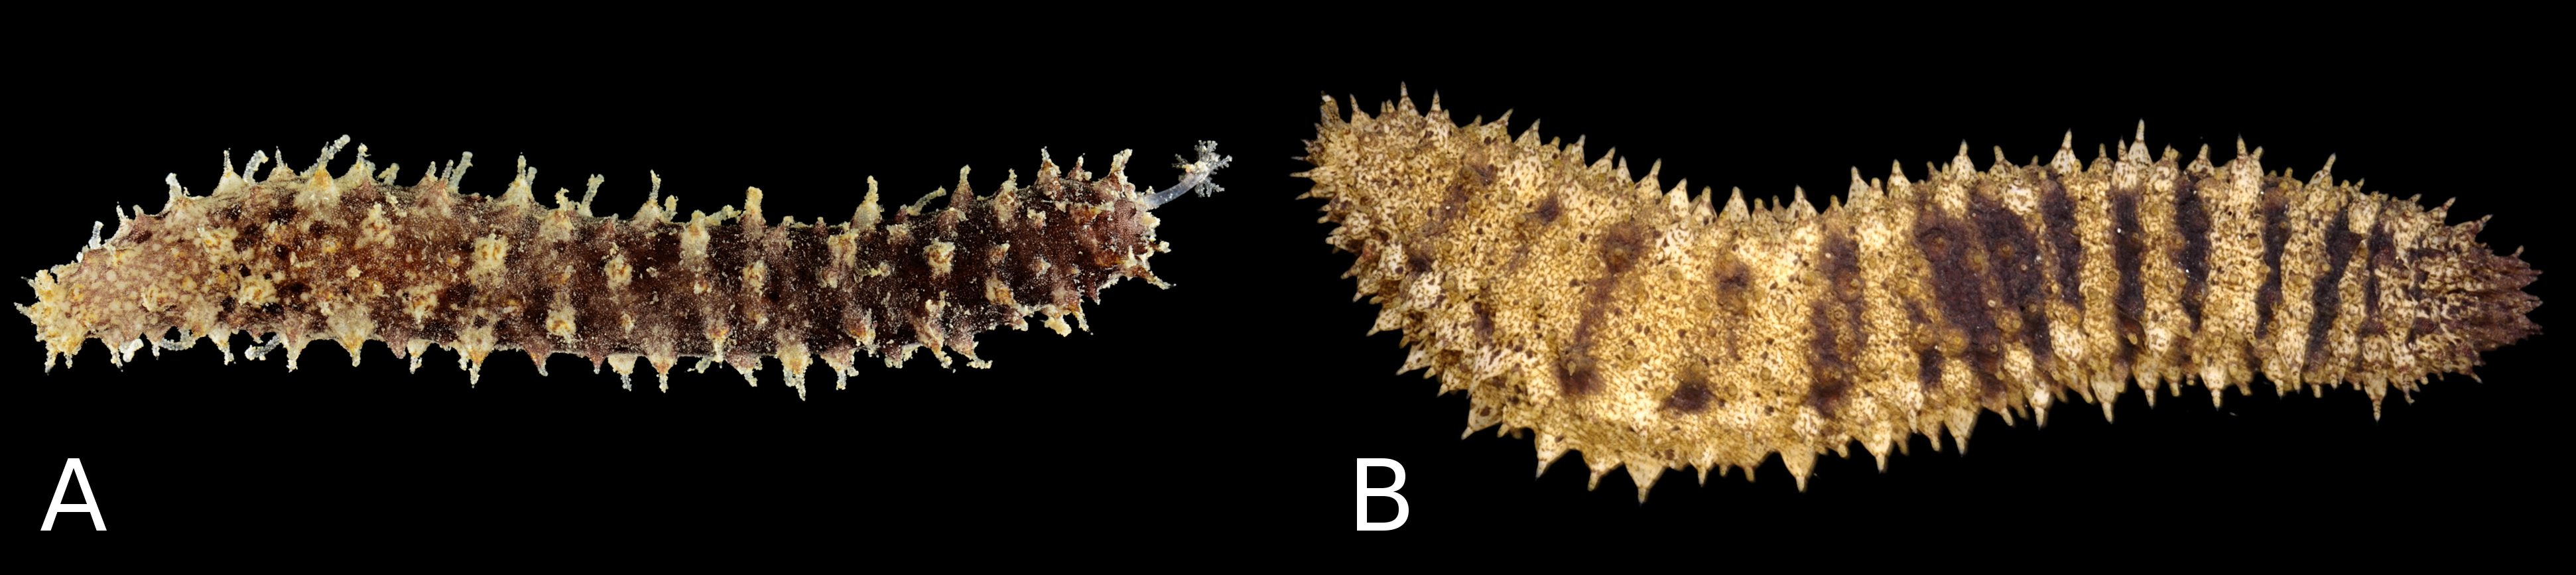
\includegraphics[width=6.5in]{figures-manual/figure-group3.jpg}
    \caption{Dorsal view of members of the ``\textit{Holothuria impatiens}''
      complex. A. WA, St Martin, UF11790; B. EP, Panama (no Voucher).}
    \label{fig:photo-WA+EP}
\end{figure}


\subsection{Species limits with *BEAST}



\begin{figure}

{\centering \includegraphics[width=\maxwidth]{figures-remake/starbeast-summary-plot.pdf}

}

\caption{Bayes factors comparing the null hypothesis (M0: \texttt{ESU1},
  \texttt{RedSea}, \texttt{Wpac}, \texttt{Hawaii} are all different species) to
  alternate models of species assignment: additional ``ghost" species added
  (oversplit), no \texttt{Hawaii} (M5), no \texttt{Wpac} (M4), no
  \texttt{RedSea} (M6), no \texttt{Wpac} and no \texttt{Hawaii} (M3), no
  \texttt{noWpac} and no \texttt{RedSea} (M2), all individuals attributed to
  \texttt{ESU1} (M1), see also Table~\ref{tab:delineationModels}. The small dots
  indicate the values obtained for independent replicated estimations, the large
  dots the mean of these values. Estimates obtained using the stepping-stone
  sampling method (on the left in blue) are consistent with the estimates
  obtained using the path sampling method (on the right in red). The horizontal
  dashed red line represents the value considered as ``very strong evidence" in
  favor of the null hypothesis according to Kass \& Raftery
  \citep{Kass1995}.}\label{fig:starbeast-summary}
\end{figure}

Both path sampling (PS) and stepping-stone sampling (SS) gave almost identical
estimates of the marginal likelihoods (Fig~\ref{fig:starbeast-summary}). The
values reported for the Bayes factors (BF) are the means of the two independent
replicates. Here, the more negative the BF, the stronger the statistical
evidence in favor of the null hypothesis specifying that \texttt{Wpac},
\texttt{Hawaii}, \texttt{RedSea} and \texttt{ESU1} are all reproductively
isolated species.

The model that included putative species identified by GMYC represented by more
than one individual, that do not differ morphologically (\texttt{Hawaii},
\texttt{Wpac} and \texttt{ESU1}) had the highest marginal likelihood
(Figure~\ref{fig:starbeast-summary}). The Bayes factors for the models that
considered \texttt{Hawaii}, \texttt{Wpac} and \texttt{RedSea} as being panmictic
with \texttt{ESU1} lent ``very strong'' support in favor of the null hypothesis
(BF=\ensuremath{-10.8}, \ensuremath{-10.5}, and \ensuremath{-24} respectively). The
model with an additional ``ghost'' species also indicated a poorer fit (BF =
\ensuremath{-5.7}), indicating that this approach did not favor a model that
included more species. The model with a random assignment of the species had the
worst fit (BF = \ensuremath{-243.5}).

% The random assignment of individuals to species led to a much lower BF (BF =
% BFrandom), indicating a strong

Similar results were obtained when COI was omitted. The differences in
likelihood were however smaller leading to $-10$ < BF < $-6$ for models that
considered \texttt{Hawaii} (BF = \ensuremath{-8.2}) and \texttt{Wpac} (BF =
\ensuremath{-9.4}) as panmictic with \texttt{ESU1} indicating ``strong''
support in favor of the null hypothesis. The BF was still below $-10$ for the
model that considered \texttt{RedSea} as panmictic with \texttt{ESU1} (BF =
\ensuremath{-19.9}).

Analyses conducted on nuclear data alone led to low BF that do not support the
null model (BF = \ensuremath{-0.2} for no \texttt{Hawaii}, and BF =
\ensuremath{-4.9} for no \texttt{RedSea}). For the model that considered
\texttt{Wpac} as the same species as \texttt{ESU1}, the BF was positive
suggesting a better fit to the data than the null hypothesis, but below the
threshold to consider the evidence ``strong'' (BF = 2.8).


\subsection{Phylogenetic relationships among the ESUs}
% TODO -- add definition of abbreviation for each ESU in figure legend if needed.

\begin{figure}
  {\centering \includegraphics[width=\maxwidth]{figures-remake/impatiens-tree-plot.pdf}}

  \caption{Bayesian phylogenetic tree of the \textit{Holothuria impatiens}
    complex. Vertical bars along the tips of the tree show the different ESUs
    found in the complex. Axis on the bottom in million
    years.}\label{fig:impatiens-tree}
\end{figure}


The phylogenetic relationships recovered with BEAST and RAxML of the species
included in the ``\textit{H. impatiens}'' complex on the concatenated alignment
were identical (Fig.~\ref{fig:impatiens-tree} and
Fig.~\ref{fig:raxml-tree}). The topology was highly supported, and the nodes
corresponding to the most recent common ancestors of the ESUs had high posterior
probabilities (> 0.99) and bootstrap values (10 out of 13 ESUs > 0.9, others >
0.8) for the Bayesian and maximum-likelihood tree respectively.

Two main clades can be distinguished that diverged approximately 10 Ma
(Fig.~\ref{fig:impatiens-tree}). The first clade (\texttt{Medit}, \texttt{WA},
\texttt{EP}, \texttt{Gala}, \texttt{ESU2}, \texttt{tiger}, \texttt{tigerRedSea})
is circumtropical and is found in the Mediterranean Sea, the Caribbean basin,
the Eastern-Pacific and across the Indo-West Pacific, including the Red Sea. The
other clade (\texttt{ESU1}, \texttt{Hawaii}, \texttt{Wpac}, \texttt{ESU3},
\texttt{gracilis}) is restricted to the Indo-West Pacific (including the Red
Sea).

The geographical ranges of the species vary considerably. Some are restricted to
an ocean basin (\texttt{Medit}, \texttt{WA}, \texttt{RedSea},
\texttt{tigerRedSea}) or an archipelago (\texttt{Hawaii}, \texttt{Gala}) but
others have ranges that encompass large sections of the Indo-West Pacific
(\texttt{ESU1}, \texttt{ESU2}, \texttt{ESU3}). This diversity of distributions
results in the co-occurrence of several species of the complex across most of
the Indo-West Pacific, and culminates in the Philippines where at least 5
species are found. More generally, at least 3 species are co-occurring in the
Northern part of the Western Pacific (the Philippines, Micronesia, Hawaiian
archipelago).

Overall, species found in the Indo-Pacific have overlapping ranges, even for
species that diverged recently. For instance, \texttt{Wpac} and \texttt{Hawaii}
co-occur with \texttt{ESU1} and diverged most recently (1.8~Ma and 2.2~Ma
respectively, Fig.~\ref{fig:impatiens-tree} and
Fig.~\ref{fig:impatiens-map-group1}).

% The phylogeny also highlights that several speciation events in the complex were
% concurrent throughout the diversification history of the complex (e.g., the first
% speciation event in each clade about 9.5 Ma).

\begin{figure}
  {\centering \includegraphics[width=\maxwidth]{figures-remake/impatiens-map-WA.pdf}}

  \caption{Distribution maps of the ESUs in Eastern Pacific and Caribbean (WA,
    Gala, EP)}\label{fig:impatiens-map-WA}
\end{figure}

\begin{figure}
  {\centering \includegraphics[width=\maxwidth]{figures-remake/impatiens-map-group1.pdf}}

  \caption{Distribution map for ESU1, ESU3, gracilis, Hawaii, RedSea, Wpac.}
  \label{fig:impatiens-map-group1}
\end{figure}

\begin{figure}
  {\centering \includegraphics[width=\maxwidth]{figures-remake/impatiens-map-group2.pdf}}

  \caption{Distribution map for ESU2, tiger, and tigerRedSea.}
  \label{fig:impatiens-map-group2}
\end{figure}


\section{Discussion}

\subsection{Species limits in the \textit{``Holothuria impatiens''} complex}

Species delineation is a complex issue and the conclusions will depend of the
characters and methods chosen. Here, using complementary approaches, combining
discovery (GMYC) and testing methods (*BEAST), we unraveled at least 13 species
within the complex ``\textit{Holothuria impatiens}'' supported by multiple lines
of evidence.

The discovery methods, based on genetic differentiation in the mitochondrial
locus COI, found putative species that require additional material to be
evaluated. In particular, three individuals characterized by divergent
haplotypes, related to \texttt{ESU1} for one, and to \texttt{ESU3} for the
others, were consistently recovered as separate species. In both cases, a single
individual was available, making it impossible to assess reproductive isolation
with *BEAST. The individual related to \texttt{ESU1} (UF8191) had the typical
color pattern of \texttt{ESU1}, with which it co-occurs and no line of evidence
seem to indicate that it could be a different species. The same situation occurs
with one of the individuals related to \texttt{ESU3} (N0027) that cannot be
differentiated from other individuals from \texttt{ESU3}. The other individual
related to \texttt{ESU3} (RUMF-ZE-0074) is small, and was dredged from 32~m in a
soft bottom bay of Kume Island, Ryukyus, Japan, a different habitat from the
typically reef-asssoicated \texttt{ESU3}. The distinct ecology and deeply
divergent sequences characterizing this individual suggest it could represent a
different species but additional material is needed to assess this hypothesis.

The combination of geography and differences in color patterns, in retrospect,
allow the differentiation of 10 species in the complex
(Figure~\ref{fig:species-limits}). Taxonomic studies of most marine
invertebrates have relied on preserved specimens. Preservation can render
delicate morphological characters, including coloration, difficult or impossible
to see, and are frequently lost or fade with time. Because hard parts are easily
preserved and their form is generally not impacted by preservation, taxonomists
often favor them to differentiate species. For instance, in sea cucumbers,
species-level taxonomy has almost entirely relied on the shape of ossicles,
microscopic calcareous secretions found in many tissues. Because ossicles show
substantial diversity and variability, whilst variation in the simple anatomy of
these animals is limited at lower taxonomic levels. Even with ossicles, until
recent decades, workers have mostly focused on those found in the body wall,
ignoring ossicles in internal structures, and have paid little attention to
intraspecific variation, typically illustrating the ossicle assemblage of a
single individual. This, in combination with the fact that several of these
species co-occur and can share the same habitat, has contributed to the failure
to recognize this diversity, and differentiate species in this complex.

Three additional species, that do not seem to be distinguishable
morphologically, and that co-occur were validated by the multispecies coalescent
statistical framework.



\subsection{Species limits with GMYC}

Despite being widely used to delineate species, the sensitivity of the GMYC
method to the factors affecting the shape of the tree used have not been
investigated thoroughly. Tree shape can be affected by biological factors or by
the type of analysis used to build the tree. Simulated data have been used to
test the influence of diversification rates, effective population sizes, and
migration rates, on the accuracy and precision of GMYC estimates
\citep{Papadopoulou2008, Esselstyn2012}. Some of the effects of the
methodological choices have been evaluated by the authors of the method
\citep{Pons2006, Monaghan2009, Fujisawa2013} and by others \citep{Talavera2013},
but the conclusions might be difficult to generalize as they depend in part on
the nature of the dataset. Other species delineation methods using sequence data
are also available (e.g., RESL \citep{Ratnasingham2013}, ABGD
\citep{Puillandre2012a}, bPTP \citep{Zhang2013}, bGMYC \citep{Reid2012}), and it
would be interesting to investigate how they perform compared to the results
obtained here.

The multiple-threshold method (mGMYC) led to higher estimates of putative
species, and was less accurate than the single-threshold method (sGMYC). We did
not find any other line of evidence that could corroborate the delineation
proposed by this approach. In particular, some of the putative species proposed
by mGMYC would split lineages that were otherwise highly supported by the
multi-locus phylogeny. The overall lower accuracy of mGMYC was also observed by
the authors of the method using a simulated dataset. They however found that the
95\% confidence set for the estimated number of putative species between sGMYC
and mGMYC were overlapping \citep{Fujisawa2013}. We observed this pattern on the
analyses using only unique haplotypes but not in the analysis that included all
sequences.

On our dataset, when analyzing all sequences, the number of putative species was
consistently 16, except for the relaxed clock with the Yule prior in which case
it was 14. The method is therefore relatively robust to prior specification on
our dataset. The 16 species delineation is the most realistic as it recovers
morphologically differentiated species that were not considered distinct in the
14 species hypothesis (\texttt{tiger} and \texttt{tigerRedSea}). Additionally,
sGMYC recovered more putative species than we can confidently recognize, since
they were represented by single individuals. This is a common pitfall of
single-locus species delineation methods, where the broad geographical sampling
of many individuals will reveal unique, divergent haplotypes that may not
represent different species. However, in our analysis, it is worth noting that
all our recognized species were apparently reciprocally monophyletic making the
GMYC approach suitable.

The combination of priors used in our study led to overestimating the number of
species when it was tested by the authors of the method \citep{Monaghan2009}. On
the other hand, Talavera et al \citep{Talavera2013} did not find any notable
differences using trees estimated with different sets of priors. Our dataset
differs from these studies by including a younger radiation, less species, and
more individuals per species.

% Esseltyn+2012 also used both all sequences & only unique, but didn't provide
% the differences in results

Talavera et al \citep{Talavera2013} did not find that using all haplotypes or
only the unique haplotypes affected the number of species estimated with the
GMYC method. Here, we confirmed the theoretical expectation that removing the
duplicated sequences overestimated the number of species and decreased the
precision of the estimates when the tree was estimated with BEAST. Removing
identical sequences in the analysis overestimates the effective population size
parameters that BEAST uses. In turn, these overestimated sizes spuriously
increase the time to coalescence for the lineages, making the estimation of the
inflection point between species- and population-level coalescent events earlier
in the tree, and more difficult to detect. This bias leads to oversplitting and
decreases accuracy. Investigating how many individuals need to be sampled to
obtain correct estimates would be worth pursuing.

GMYC was developed with the intent of automating the estimation of the number of
species from large-scale single-locus sampling efforts, particularly from
environmental samples. In this context, a reasonable amount of inaccuracy or
imprecision from the true number of species may be acceptable. The advantage of
the method, namely providing a rapid and objective assessment of the number of
species, outweighs the possible deviations from the true value. However, in the
context of a taxonomic study where the goal is to identify species limits among
a few hundred individuals, the factors affecting tree shape need to be
considered, and additional lines of evidence need to be included to validate the
putative species delineated \citep{Marshall2011a, Esselstyn2012}.

\subsection{Species limits with *BEAST}

The statistical framework offered by *BEAST that compares alternative models of
species assignment seems a promising venue to investigate species limits, when
other lines of evidence are equivocal (e.g., \citep{Grummer2014,
  Satler2013}). The requirement to assign specimens to species \textit{a priori}
can however be challenging. When morphological evidence is scarce, and deeply
divergent lineages are recovered with genetic data, circularity is introduced
when the same data is used to recognize species, and to provide statistical
support for these species. Here, COI was used to assign species to individuals
for putative species that could not be differentiated morphologically.

The confounding effects of using COI to formulate the species hypotheses and to
test species limits can stem from: (1) the information contained in the
nucleotides forming the locus, and (2) from the absence of recombination in
mitochondrial DNA. We attempted to evaluate the relative contribution of these
confounding effects by conducting the analyses without COI and without
mitochondrial respectively. The results for the analyses conducted without COI
were qualitatively similar to the analyses performed with this locus, but the
statistical evidence in favor of the hypothesis considering these closely
related lineages as different species, was weaker. There was no statistical
evidence supporting this hypothesis when the analysis was conducted on nuclear
data alone, owing to the low differentiation in these loci for the putative
species tested by the models. These results suggest that the remaining of the
mitochondrial loci used in our study also favor the null hypothesis, but
additional independent nuclear loci with enough differentiation to tease out
these species are needed.

Another potential issue with assigning species to individuals based on their COI
sequences, is that they may not reflect species limits because of introgression
or incomplete lineage sorting. Recently diverged species might still be poly- or
paraphyletic in their COI genealogy making species assignment
inaccurate. Inaccurate species assignment can potentially be detected from the
population sizes estimated by *BEAST that will be unusually high
\citep{Leache2013, Drummond2014}. This would however require to analyze more loci
than in the present study to obtain accurate estimates of population sizes
\citep{Heled2010, Harris2013}. Determining how the Bayes factors will behave if
the null hypothesis is misspecified remains to be investigated.

\subsection{Species limits and coloration}

Before the confirmation by molecular methods that differences in coloration were
relevant to differentiate closely related species, marine invertebrate
taxonomists have been reluctant to consider species defined solely by
differences in coloration \citep{Knowlton1993}. Although variation in coloration
within ``\textit{H. impatiens}'' has been noticed by previous workers, and some
unusual color morphs were described as sub-species by Clark \citep{Clark1921,
  Clark1938}, the focus on ossicle shape to distinguish sea cucumber species has
led to an underestimation of the diversity in this group.

The purpose of coloration in sea cucumbers has not been explored but since
species can be distinguished based on their color patterns, natural selection
may play a role in its evolution. Color patterns have been documented to be
diagnostic of species limits in crustaceans \citep{Malay2010}, nemerteans
\citep{Knowlton1993}, fish \citep{McMillan1999}. In some of these cases, the
association between color patterns and species limits is maintained by assortative
mating (fish \citep{McMillan1999}, crabs \citep{Detto2007, Baldwin2012}). Given
that most sea cucumbers inhabit cryptic habitats and do not possess
image-forming eyes, the mechanisms maintaining a tight association between
coloration and species identity needs to be investigated.

While some species of ``\textit{H. impatiens}'' harbor slight variations of the
typical color pattern characterizing the complex, others deviate from it and are
polymorphic. For instance, \texttt{ESU2} has two color morphs: a common color
pattern that occur throughout the range of the species, and one restricted to
the Western Indian Ocean (Nosy B\'{e}, Madagascar and R\'{e}union Island). Both
\texttt{gracilis} (alternate morph in the southern part of the Great Barrier
Reef) and \texttt{ESU1} (alternate morph found in Lizard Island, Australia;
Hawaii; and Guam) are also polymorphic.  Interestingly, these alternate color
morphs are similar for the three species (uniform chocolate brown background
with white to yellowish tubercles), and could result from allelic polymorphism
shared across species in genes involved in the pigmentation pathways (as in
albinism or melanism), or from convergent selection. These two hypotheses are
not mutually exclusive. Furthermore, since coloration seems indicative of
species limits, these alternate color morphs could also represent additional
cryptic lineages.

% TODO -- add pictures of alternate color morphs

Even though, there is no genetic differentiation in the markers used in this
study to distinguish individuals exhibiting these alternate color patterns,
studies in fish indicate that color differentiation between incipient species
might precede any genetic signal (e.g., \citep{McMillan1999,
  Gaither2014}). Additional genetic data (microsatellites, SNPs) can test
whether they represent distinct evolutionary lineages.


\subsection{Geographical distributions}

The geographical ranges of the species vary considerably, and a diversity of
processes seem to best explain their present distributions. Interestingly no
speciation along a continental margin is observed in the complex.

The close phylogenetic relationship of \texttt{WA} with \texttt{EP} and
\texttt{Gala} indicates that the closure of the isthmus of Panama led to the
isolation of the species in the two basins.

The estimated ages of \texttt{Medit}, and the two Red Sea species are older
(8.4-10.5 My, 1.1-1.7 My and 3.2-4.1 My respectively) than the last salinity
crises characterizing these seas (\textit{c.} 5 My for the Mediterranean
\citep{Hernandez-Molina2014} and potentially as early as \textit{c.} 19,000 years
ago for the Red Sea). This, in combination with the occurrence of these species
outside their basins (\texttt{Medit} is known from Portugal and the Canaries;
and both Red Sea species from Djibouti) indicate that these species invaded
these seas recently and found refugia at the periphery of these basins during
the salinity crises \citep{DiBattista2013}. It is also interesting to note that
the age of divergence for the two species from the Red Sea do not coincide
suggesting that different events were responsible for the geographic isolation
of these populations.

\texttt{tiger} and \texttt{tigerRedSea} are nocturnal species found on the reef
slope. They are very sensitive to light, and retract quickly, deep into the reef
matrix if a diver shines light on them. These species are known from a handful
of individuals, and it is possible that their ranges are larger than what is
reported here.

For species with wide ranges the causes of population divergence are less
obvious, and the current distributions may not reflect species distributions at
the time of speciation. The two most widespread species (\texttt{ESU1} and
\texttt{ESU2}) are sympatric or parapatric with their closely related species,
and both form the terminal clades in their respective radiations. This pattern
suggests that these species were the sequential source of the peripheral species
\citep{Malay2010}.

The lack of genetic differentiation between the Indian and Pacific Oceans for
the species of the complex that occur on each sides of the Indo-Pacific barrier
(IPB) is noteworthy. The IPB results from the restricted seaway between the
Sunda and the Sahul shelves. During glaciation events, when sea levels were
100+~m below present level, only a narrow channel connected Indian and Pacific
Oceans. In a recent literature survey, 15 out of 18 species of fish and
invertebrate investigated showed genetic differentiation across the IBP
associated with these low stands events \citep{Gaither2010}. Additionally, the
genetic diversity of \texttt{ESU1} is low: among the 61 individuals sequenced,
we found a total of 18 haplotypes, with the 3 most common haplotypes found in 40
individuals. Finally, both Marquesas and Oman, characterized by distinct
ecological conditions from the rest of the Indo-Pacific hypothesized to increase
the speed and probability of divergence, harbor the most widespread haplotype
suggesting recent colonization of these peripheral areas to \texttt{ESU1}'s
range. Together, these lines of evidence suggest a recent geographical expansion
for the widespread species in the complex, but more analyses to confirm this
hypothesis are needed.

Differences in the geographical ranges for some of the species might be
explained by differences in habitat preferences. For instance, \texttt{tiger} is
only found in the oligotrophic shallow waters of Micronesia and Hawaii, while
\texttt{ESU3} and \texttt{gracilis} appear restricted to continental areas. For
instance, \texttt{ESU3} found in Madagascar and Tanzania, was not encountered in
the oceanic Mayotte or Scattered islands. We lack data to evaluate the role
played by the ecology of the species in the diversification process and the
co-existence of multiple species in sympatry.


\subsection{Rates of secondary sympatry}

Local diversity results from the accumulation of species that are reproductively
isolated. Because reproductive isolation is most commonly initiated in allopatry
\citep{Coyne2004}, understanding how quickly species can be found in sympatry
after diverging in geographical isolation is key to gain insights into the
temporal dynamics of local diversity.

The restriction of marine invertebrates to ``oceanic'' and ``continental''
habitats has been documented for a range of organisms (e.g., land snails
\citep{Paulay1994}, marine snails \citep{Abbott1960, Reid2006b, Williams2011},
hermit crabs \citep{Malay2010}), and a variety of biotic and abiotic factors may
explain this pattern (reviewed in \citep{Malay2010}). Interestingly, clades
associated with continental habitats are characterized by much faster rates of
secondary sympatry than species associated with insular habitats in both
vertebrates (e.g., \citep{Taylor2005, Hodge2012}), and invertebrates (e.g.,
\citep{Meyer2005-evolution, Malay2010, Williams2011}). As a result, closely
related species typically show strict allopatric distributions in oceanic
setting (e.g., as in \citep{Meyer2005-evolution}) but often occur in sympatry
along continental margins (e.g., \citep{Williams2011}). Differences in rates of
secondary sympatry vary across taxa but are faster in continental settings. For
instance, in the wrasse \textit{Anampes} sympatric sister species in continental
setting diverged 600 ka ago, while the most closely related sympatric species in
oceanic setting shared a common ancestor more than 10 Ma ago
\citep{Hodge2012}. In the turbinid \textit{Lunella}, none of the 7 lineages
inhabiting oceanic islands that have diverged more than 15 Ma occur in sympatry
while sister species found along the coastline of Oman have diverged 5 Ma
\citep{Williams2011}.

The ``\textit{Holothuria impatiens}'' complex shows a strickingly different
pattern, and \texttt{ESU1}, \texttt{Hawaii} and \texttt{Wpac} are, to our
knowledge, the fastest documented examples of speciation for a broadcast spawner
invertebrate in an oceanic setting (\texttt{ESU1} and \texttt{Hawaii} diverged
less than 2~Ma, and \texttt{ESU1} and \texttt{Wpac} about 2.5~Ma). Thus, species
have been able to evolve reproductive isolation rapidly, and differ enough
ecologically to allow for co-existence. In other words, the temporal dynamics of
diversification in some oceanic species of the ``\textit{Holothuria impatiens}''
complex is similar to what is observed for species occurring in continental
settings.

Gamete recognition proteins (GRPs) play an important role in driving
reproductive isolation in many free spawning organisms, such as sea urchins
\citep{Levitan2006, Lessios2011} and gastropods \citep{Hellberg2000}. For
instance, strong positive selection has been detected in the GRPs between
closely related species of sea urchins in sympatry but not in allopatry
\citep{Geyer2003}, suggesting the role of these proteins in maintaining species
limits.  GRPs have not yet been identified in sea cucumbers but bindin is known
from sea urchins \citep{Lessios2011} and sea stars \citep{Patino2009} which
indicates that it is plesiomorphic in the clade that sea cucumbers emerged
from. They could explain how species in the ``\textit{H. impatiens}'' complex
acquired reproductive isolation quickly.

Hellberg \citep{Hellberg1998} proposed that climatic fluctuations isolate
populations temporarily leading to speciation (transient allopatry), and as
climatic conditions change, species shift their ranges. In continental settings,
these shifts will lead to species coexistence as their distributions are
constrained by the one dimensionality of the coastline. In insular conditions,
however, these shifts in species distributions could be accompanied with the
colonization of new islands and species could remain allopatric. Another
difference is that in the continental setting the environmental conditions will
vary continuously along the coast. Therefore, if species are adapted to
different temperatures, the temperature gradient along the coast will allow
species to overlap. However, in an insular setting, the absence of available
habitat between the islands restricts the distribution of the species. These
hypotheses could explain why most species remain allopatric for long periods of
time and are restricted to archipelagos (as observed for \texttt{Hawaii} and
\texttt{Gala}): rare migrants fail to colonize as local adaptation to
environmental conditions render them maladapted to new islands. This model
implies niche conservatism: species are narrowly adapted to a particular
environment. The predictions of this model would suggest that \texttt{ESU1} has
broadened its niche to allow the colonization of the range of \texttt{Hawaii}
and \texttt{Wpac}.

% TODO -- need drawing for hypothesis here

% TODO -- alternatively, it migh

% We hypothesize that \texttt{Wpac} and \texttt{Hawaii} are the consequences of
% peripatric speciation events where a combination of selection to local
% environmental conditions and low effective population sizes have led to rapid
% reproductive isolation. Adaptation to local environmental conditions for Wpac
% and Hawaii is suggested by their restricted geographical ranges. Small effective
% population sizes are suggested by the low levels of heterozygoty observed for
% these species as well as the reciprocal monophyly observed for all species at
% the majority of the loci. Additionally, echinoderms, as other marine organisms,
% have life-history characteristics that make them prone to low effective
% population sizes: strong bias in reproductive success, size-dependent fecundity
% \citep{Gonzalez2008a}. Additionally, echinoderms are renown to experience drastic
% population sizes fluctuations \citep{Uthicke2009} which contributes further to
% reduce effective population sizes. If low effective population sizes might limit
% a species adaptive potential, the low genetic diversity will facilitate the
% fixation of alleles that might contribute to rapid acquisition of reproductive
% isolation.

\subsection{Future directions}

A shortcoming of the approach used in this study is that the results might be
strongly influenced by the loci that harbor the most genetic differentiation,
here the mitochondrial data. A recent extension of these methods, using
single-nucleotide polymorphisms across the genome \citep{Leache2014} would allow
the confirmation of the species delineated in this study.

\section{Conclusions}

This study showed that the widespread, common and well known sea cucumber,
\textit{Holothuria impatiens} is actually a complex of at least 13
species. This estimate is conservative as additional lineages that could not be
fully evaluated were also unraveled.

The multispecies coalescent framework allows the investigation of species limits
in situations where evidence might have been inconclusive in the past. It is now
possible to investigate species limits in groups that show some level of genetic
differentiation but no morphological differences. The re-evaluation of species
limits, and a better accuracy in the estimation of the divergence times, may
improve our understanding of the speciation process by revealing new patterns
and generating new hypotheses. Here, we showed that some species in this complex
are characterized by the most rapid rate of secondary sympatry documented for a
broadcast spawner in an oceanic setting. These results would need to be
confirmed with genetic data that capture a larger fraction of the genome.

% More generally, we unraveled an unusual pattern where the range of most species
% of this complex are broadly overlapping.

% \textit{Holothuria impatiens} is not an isolated case. Other marine organisms
% also hide substantial cryptic diversity.


% Many cryptic species = change in patterns of biodiversity
% - find examples of other species that show similar patterns indicative of small
%   scale endemism
% - potential to redefine hotspots
% -

% possibly easier to detect because faster to achieve reciprocal monophyly.

% Bowen et al \citep{Bowen2013} suggest that sympatric speciation is possible among
% marine organisms. In particular, they cite Rocha \citep{Rocha2008} that
% investigated patterns of speciation among grunts (\textit{Haemulon}) in the
% Caribbean and the Eastern Pacific that show closely related species occurring in
% sympatry. Authors in this study invoke the possible role of the sounds members
% of this genus produce in assortative mating.


%% Geography of speciation
% one of the difference between marine and terrestrial speciation is that the
% dissociation between geogrpahical isolation and absence of gene flow is
% probably stronger in the sea.

%% New genomic methods will allow better characterization of demography of the
%% species, and finer understanding of what happened in this complex.

%% Possible scenarios:
% - selection under uniform selection: different mutations are fixed under same
% environment in populations evolving allopatry, alternate mutations cause
% postzygotic isolation by DM incompatibilities (Sobel et al 2010)

%% "Geographic ranges are the product of both ecological and historical factors"
%% "Historical processes leading to allopatry will often give way to ecological
%% processes as populations adapt to different habitats."
%% (Sobel et al 2010)

% According to \citep{Renema2008}, the modern IWP fauna has its origin in the
% Miocene. Generation of hotspots associated with tectonic events, so importance
% of abiotic factors.

% relationship between reproductive isolation and genetic
% differentiation for sympatry and allopatric species (review
% Rabosky&Matute PNAS).


%% Short review on how the rates of secondary sympatry is much faster in
%% impatiens compared to other examples.
% - in Quenouille+2011, fish take at least 4 MYa to reach secondary sympatry
% - Look into \citep{Lessios1999} to see how the timing in Eucidaris compares to
% the one H. impatiens

%% Knowlton 2000 says that for alpheids, all species are older than
%% closure of isthmus of Panama (except for some fish, and snails
%% [examples given are however, from continental setting])
%% - see Puritz to see what they say exactly about timing of speciation.

%% Traditionally 2 views:
%% - small populations -- speed up divergence?
%% - local adaptation -- role of ecology and interplay with selection on GRPs


% In the case of founder effects (parapatric speciation), where a small population
% establishes itself in the periphery (and therefore being connected with limited
% gene flow) from the ancestral population, the genetic diversity of these
% individuals will be limited. The success of the establishment of this peripheral
% population will depend on its density and its genetic make up that will allow
% for its local adaptation to ecological conditions in the new environment, and
% will ensure the compatibility of the genotypes for the gamete recognition
% proteins. In sea urchins, Levitan \& Ferrel have shown that at low density,
% males and females with identical genotypes for bindin, have higher reproductive
% success \citep{Levitan2006}. Therefore, if the pool of individuals that colonized
% the peripheral location harbors genotypes that are non-representative of the
% ancestral populations, and/or if the genotypes are in linkage-disequilibrium
% with genes being selected for in the new environment, GRPs will drive divergence
% between populations, leading to reproductive isolation.



%% From Doorn et al 2009 "Once a mating preference for locally adapted
%% partners has evolved, sexual selection reinforces assortative mating and
%% lowers the fitness of hybrids." How does density dependence in fecundation
%% success interplays with/changes this statement?
%% One can imagine that if particular genotype associated with high fitness in
%% particular habitat, abundance is higher,

%% Review papers on GRP to see if they are considered a Fisherian sexual
%% selection trait




% Speed of speciation/secondary sympatry
% - how they managed to accomplish that
% - signature of population expansion?
% - implication for identification of geographical boundaries in distribution
% - role of pre- and post-zygotic barriers
% - role of selection?

%\section{Conclusions}

% museum collections need to be future proof


% \section{Acknowledgments}

% Stolarz
% DDIG
% iDigBio
% NSF PEET
% collectors
% CIPRES portal.
% UF HPC, HiPerGator.
% wesanderson
% knitr
% polymode + ESS

\pagebreak

\bibliographystyle{sysbio}

\bibliography{impatiens_nourl}

\pagebreak

\section{Supplementary materials}

\subsection{Supplementary figures}

\begin{figure}
{\centering \includegraphics[width=\maxwidth]{figures-remake/loci-coverage-plot.pdf}}

\caption{Representation of the loci sequenced for each individual included in
  the analysis.}\label{fig:loci-coverage-plot}
\end{figure}



%% raxml tree
\begin{figure}
  {\centering \includegraphics[width=\maxwidth]{figures-remake/raxml-tree.pdf}}
  \caption{Maximum-likelihood phylogeny for all concatenated loci',
    fig.cap='Maximum-likelihood phylogeny for all concatenated loci estimated
    using RAxML with a GTR+G model for each partition. Black circles represent
    bootstrap values $\geq$ 90, red circles bootstrap values $\geq$
    80. Colored vertical bars represent consensus
    ESUs.}\label{fig:raxml-tree}
\end{figure}

%% locus trees
\begin{figure}
  {\centering \includegraphics[width=\maxwidth]{figures-remake/per-locus-trees.pdf}}
  \caption{Maximum-likelihood genealogies (unrooted) for each locus
    reconstructed using RAxML with a GTR+G model of molecular evolution for each
    partitions. Black circles on the nodes indicate bootstrap values $\geq$ 80
    based on 500 replicates. Terminals are colored based on their ESU. ``mtDNA"
    is the concatenation of ATP6, COI, 16S; ``rDNA" is the concatenation of ITS
    and LSU.}\label{fig:per-locus-trees}
\end{figure}


%% gmyc tree
\begin{figure}
  {\centering \includegraphics[width=\maxwidth]{figures-remake/gmyc-tree-all-sequences.pdf}}
  \caption{Position of the species delineated with GMYC on COI genealogies
    estimated using various priors with BEAST. Each color corresponds to a
    different putative species.}\label{fig:gmyc-tree-plot-allSeq}
\end{figure}

\begin{figure}
  {\centering \includegraphics[width=\maxwidth]{figures-remake/gmyc-tree-unique-sequences.pdf}}
  \caption{Position of the species delineated with GMYC on COI genealogies
    estimated using various priors with BEAST. Each color corresponds to a
    different putative species.}\label{fig:gmyc-tree-plot-uniqSeq}
\end{figure}


\clearpage

%% specimen table

\subsection{Supplementary Tables}

\begin{table}[h]
  \centering
  \caption{Partition table. The subscript number corresponds to
    the to the codon position in the alignment. The ``real'' codon position is
    offset by 2 for COI, H3a and ATP6 (i.e., COI$_1$ is 3rd codon position)}
  \begin{tabular} { l l l }
    \hline
    Partition & Model   & Loci              \\
    \hline
    1      & GTR+I+G    & 16S, ATP6$_2$     \\
    2      & HKY+I+G    & ATP6$_1$, COI$_1$ \\
    3      & HKY+I+G    & ATP6$_3$, c0775   \\
    4      & GTR+I+G    & c0036             \\
    5      & GTR+I+G    & COI$_2$, H3a$_2$  \\
    6      & HKY+I      & COI$_3$           \\
    7      & HKY        & H3a$_1$, LSU      \\
    8      & JC         & H3a$_3$           \\
    9      & HKY+G      & ITS               \\
    \hline
  \end{tabular}
  \label{tab:sm-partitions}
\end{table}


Specimen Table in Supplementary Material (see
\textsf{supp-materials-remake/specimen\_table.csv}). \label{tab:specimen-table}

% <<specimen-table, eval=TRUE, echo=FALSE, results='asis'>>=

% @


\end{document}

%% Notes about the biology of the species
%% - EP: discharge Cuv tubules \citep{Bakus1974}, ``relatively very active''
%% \citep{Bakus1974},
%% - Egypt: tables appear earlier than buttons in juveniles, look for pl.8 fig4-5,
%% and pl.9 2 in Savigny \citep{Mortensen1902}10.1111/j.1096-3642.1926.tb00326.x

%% READ \citep{Cutress1996}, seems like there is a lot of information about
%% ontogenetic changes in the shape of the ossicles.
%% ``Buttons in OM dermis of the 195 mm specimen from Ceylon, however, are
%% distinctly smaller.''


% ESU2: Easily recognizable because of (1) yellow tentacles and tube feet, (2)
% round tubercles, (3) light gray/purplish background with white areas, and dark
% stripes in the anterior ends, progressively becoming blotches towards posterior
% end, clearly marked salt-and-pepper coloration typically more prevalent towards
% posterior end. In some specimens (most common in juveniles), coloration
% uniformly dark purple, or black, with only tube feet appearing yellow. Cuvierian
% tubules, rarely released, long, relatively wide (about 2mm in diameter), white
% with a light blue tint.






%% Misc
% look into splitstree (already installed into ~/Software folder), this allows
% to test for the robustness of signal in minimum spanning tree (see Volger+2012
% for details)

% look into \phi_{ST}, Fu's F, Tajima's D (reading the Arlequin manual)

% If ecological differences between these incipient species evolve through
% competition upon secondary sympatry to allow for coexistence, one would expect
% species in continental settings to differ ecologically more than species
% occurring in insular setting.


%%%


% The development of genetic data and its application to species identification
% have allowed the discovery of many species complexes. The DNA barcoding approach
% of using an easy-to-amplify single locus to delineate species provides a
% promising venue to speed up biodiversity documentation. Ideally the analysis of
% the genetic data should delineate the biological species accurately with little
% or no subjectivity, so that the process can be automated and used on large
% datasets. However the biological processes generating the genetic
% differentiation that can be used to delineate species, depends on a variety of
% other factors than reproductive isolation that a single locus cannot
% capture. Nonetheless, threshold based methods (e.g. \citep{}) or other methods
% developped \citep{Pons2006}, \citep{Monaghan2009} to detect species limits are
% relatively succesful. While the possibility of detecting accurately species
% limits from a single marker remains contentious, using multiple lines of
% evidence to assess species limits in species complexes detected from
% single-locus dataset is widespread. The development of integrative taxonomy
% which uses multiple lines of evidence to delinate species has recently seen more
% formal development in how to determine the species limits based on available
% evidence. The most recent developments favor finding a biological explanation
% behind contradictory lines of evidence \citep{Schlick-Steiner2010}. For genetic
% data, recent developments in Bayesian statistics allow for integrating genetic
% signal from a variety of markers by invoking the multi-coalescent process and
% also compare competing models.

%%%%%%%%%%%%%%%%%%%%%%%%%

% Inferring the mode of speciation from current distributions can be misleading
% because species distributions are dynamic and are especially influenced by
% large-scale environmental changes. Glacio-eustatic sea level fluctuations have
% had an important impact on shallow marine habitats because 100+~m amplitude
% exceeds the depth range of most littoral species, and they recurred with
% \char`~10$^4$-10$^5$ year periodicity during the late Tertiary and
% Quarternary. These fluctuations have led to important habitat modifications and
% changes in oceanic current patterns with consequences in connectivity,
% population sizes and species ranges. These changes have made species
% distributions in the Pacific highly dynamic (\citep{Paulay1990}) and are, in most
% cases, too recent compared to the time frame needed for speciation.
% % However, speciation can be very rapid, e.g., Asterinid from NSW Byrne2012
% For instance, the latest minimum sea level (120 to 135~m below present) was
% 18,000 years ago. During this period, circulation between Pacific and Indian
% Oceans was significantly restricted, the Red Sea was most likely disconnected
% from the Indian Ocean, and the South China Sea was nearly land-locked
% (\citep{Veron1995}). Therefore, current distribution patterns  only
% partially reflect the biogeographical context under which the modern
% reef-associated fauna diversified. This is illustrated by the observation that
% modern faunal breaks in the reef fauna are only poorly correlated with
% present-day conditions, but are strongly associated with geological features
% \citep{Keith2013,Pellissier2014}.

% The consequences of sea level fluctuations on the populations can be apparent in
% the present genetic diversity and structuring. For instance, during low sea
% stands the connectivity between the Indian and Pacific oceans was reduced,
% providing repeated opportunities for population divergence between these ocean
% basins. While some species show substantial divergence in their mitochondrial
% DNA (e.g., xxxxxx), many others (including the most widespread form of
% \textit{Holothuria impatiens}) show little genetic structuring across this
% area. Such lack of pattern can be the result of (1) maintained connectivity
% during these low sea stands, as both oceans were still connected
% (\citep{Voris2000}); (2) one of the two lineages was lost because of local
% extinction or selective sweep; (3) the species recently expanded its ranges
% and colonized one of the basin recently.



% Based on the precept that species are defined on the criterion of reproductive
% isolation, three processes operating at different rates are interacting during
% speciation: (1) acquisition of reproductive isolation, (2) morphological
% differentiation, (3) genetic differentiation. In many cases, these three
% processes can be independent making species delineation challenging. For
% instance, broadcast spawning marine invertebrates for which reproductive
% cohesion is maintained behaviorally
% %(e.g., spawning aggregations cukes?,
% %lobsters? \citep{}, spawning based on environmental clues corals? \citep{})
% and biochemically (e.g., gamete recognition proteins \citep{Hellberg2000}),
% selection on these traits is unlikely to drive morphological differentiation
% among closely related species \citep{Knowlton1993}. Similarly, barcoding markers
% evolve typically neutrally and the time taken for them to show enough
% differentiation to be recognized as different species will depend on effective
% population sizes or DNA repair mechanisms (in absence of introgression) that
% will also be independent of the species identity.

% The failure to distinguish reproductively isolated species can stem from either
% the choice of an inappropriate set of characters to distinguish species
% otherwise morphologically variable, or from the absence of variation in
% morphology but differentiation in other traits (e.g., ecology, chemical cues)
% allows them to remain reproductively isolated

% \subsection{Taxonomic consequences}

% The \textit{H. impatiens} complex belongs to the subgenus \textit{Thymiosycia}
% of which it is the type species. However, except for \textit{H. gracilis}, no
% other species currently included in this subgenus shows any affinity with the
% ``\textit{H. impatiens}'' complex. The subgenus \textit{Thymiosycia} therefore
% needs to be redefined to only include the species of the \textit{H. impatiens}
% complex. Based on species descriptions, no name can be applied to the species in
% the complex, and all will need to be described formally.

% As the type locality for \textit{H. impatiens} is the Northern Red Sea, based on
% its description and the drawing accompanying it, our results indicate that this
% species (RedSea here) is actually restricted to the Red Sea.

% As a consequence, all the studies on the biology of ``\textit{H. impatiens}''
% were in most cases based on one or more species of the complex. In some cases
% the identity of these species can be guessed as the locality is indicated and
% only one species is known from there, but in other cases it cannot since the
% locality is missing (e.g., \citep{Hampton1958,Hampton1959}) or several species
% are known from the area (e.g., \citep{Roberts1982,Cutress1996}).


%% Diversification of the complex is really ~20 MY really fits with idea that
%% most of the reef-associated fauna diversified with corals see citations
%% within Williams et al 2011.
